\chapter{Käyttöönotto}

\section{Tyyppiannotaatiot}

Tyyppijärjestelmä voi päätellä muuttujan sallitun tyypin automaattisesti
tai kielen syntaksin tarjoamien eksplisiittisten tyyppimäärittelyjen
perusteella. Kaikki kolme tässä tutkielmassa esiteltyä JavaScriptin staattiseen
tyyppitarkastukseen tarkoitettua työkalua päättelevät muuttujien tyyppejä
automaattisesti, mutta vaativat paikoitellen myös eksplisiittisiä määrityksiä.
Closure-kääntäjä lukee
tyyppimääritykset JSDoc-tyylisistä dokumentaatiokommenteista \cite{annotatingJSforClosure}.
\begin{lstlisting}[caption={Esimerkki Closure-annotaatiosta funktiolle},label={lst:ostoskorin_hinta_closure}]
/**
* @param {!Array<Ostos>} ostokset
* @return {number} Ostosten yhteenlaskettu hinta
*/
function ostoskorinHinta(ostokset) {
  let summa = 0;
  for (const ostos of ostokset) summa += ostos.hinta;
  return summa;
}
\end{lstlisting}
Listauksessa \ref{lst:ostoskorin_hinta_closure} \inlinecode{ostoskorinHinta}-funktion
tyyppimäärittely on toteutettu sen yläpuolella olevilla kommenteilla, jotka määrittävät
tyypin \inlinecode{ostokset} parametrille sekä funktion palautusarvolle.
TypeScript ja Flow puolestaan jatkavat ECMA-262-spe\-si\-fi\-kaa\-ti\-o\-ta
erityisellä syntaksilla tyyppien eksplisiittistä määrittämistä varten. 
\begin{lstlisting}[
  float,
  caption={Esimerkki Flow tai TypeScript annotaatiosta funktiolle},
  label={lst:ostoskorin_hinta_flow}
]
function ostoskorinHinta(ostokset: Ostos[]): number {
\end{lstlisting}
Flow ja TypeScript -esimerkissä \ref{lst:ostoskorin_hinta_flow}
tyyppiannotaatiot ovat osana koodia, mikä
tekee ohjelmasta yhteensopimattoman tavallisen JavaScriptin kanssa. Ohjelma
on käännettävä JavaScriptiksi ennen suorittamista. Annotaatioiden
syntaksi ja merkitys eivät myöskään ole välttämättä suoraan selviä
JavaScript-ohjelmoijalle, joka pahimmassa tapauksessa voi kokea lisätyt
tyyppimäärittelyt vaikeasti luettavina. 

Closuren annotaatiot on sijoitettu kommentteihin, joten niillä ei ole
ajonaikaista vaikutusta ja ohjelma on täten sellaisenaan hyväksyttävää
JavaScriptiä. Toisaalta tyyppiannotaatioiden määrittely kommenteissa voi
olla runsassanaista ja hankalaa, mikä kasvattaa niiden kirjoittamiseen vaadittua
työmäärää \cite{TypeScriptSpec, TypeScriptatBuild}.

Aiemmassa esimerkissä esitelty tyyppi \inlinecode{Ostos} pitäisi
määritellä Closurea varten muiden annotaatioiden tapaan dokumentaatiokommentteja käyttäen:

\begin{lstlisting}[
  caption={Uuden tyypin määrittely Closuren kommenttisyntaksilla},
  label={lst:closure_typedef}
]
/**
* @typedef {{
*   nimi: string,
*   hinta: number
* }}
*/
let Ostos;
\end{lstlisting}
TypeScript ja Flow tarjoavat käännösaikaisen tyypin (type alias)
määrittelyyn tiiviimmän ja helppolukuisemman syntaksin \cite{TypeScriptSpec}:
\begin{lstlisting}[
  caption={Uuden tyypin määrittely TypeScriptissä tai Flow'ssa},
  label={lst:ts_flow_type_alias}
]
type Ostos = {
  nimi: string;
  hinta: number;
};
\end{lstlisting}
Tällainen tyypin määritteleminen vaikuttaa ainoastaan käännösvaiheen
tyyppitarkastukseen, eikä määrittely tuota tietorakenteita tai muuta
sisältöä suoritettavaan JavaScript-ohjelmaan.

\section{Käännösprosessi}
\begin{figure}[!htb]
\centering
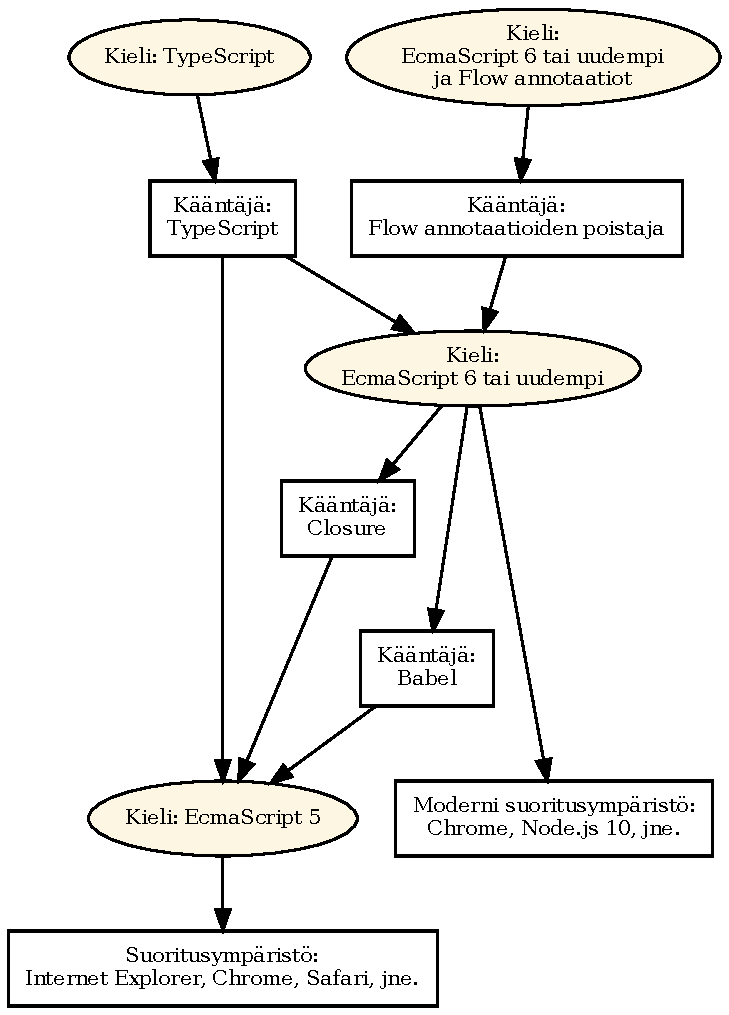
\includegraphics[width=0.8\textwidth]{images/compilation.pdf}
\caption{Vaihtoehtoisia käännösprosesseja}
\label{fig:compilation}
\end{figure}
JavaScriptillä kirjoitettua koodia ei tavallisesti tarvitse
erikseen kääntää ennen suoritusvaihetta. JavaScriptiä suorittava ohjelma,
esimerkiksi selain, tulkkaa EcmaScript-standardin mukaista koodia
sellaisenaan tai \textit{JIT-kääntää} \cite{MozillaJIT}
sen optimoituun muotoon automaattisesti
suorituksen ohessa. TypeScript- tai Flow-annotoitu koodi ei kuitenkaan
ole validia JavaScriptiä, eikä selain tai muu JavaScriptia suorittamaan
suunniteltu ohjelma tavallisesti osaa sellaista koodia käsitellä.
Näinollen TypeScript tai Flow-annotoitu koodi on välttämätöntä kääntää muotoon jossa
annotaatiot on poistettu ja jäljellä on enää standardinmukainen JavaScript.

Kääntämisen tarve vaikuttaa ohjelman kehitysprosessiin.
Koska JavaScriptin käyttäminen ei normaalisti vaadi erillistä
käännösvaihetta, useissa projekteissa ei ole sellaista käytetty. Koodin
minimointi ja muu optimointi on ollut parhaiden käytäntöjen mukaista jo
tovin, mutta tällaiset koodinkäsittelyt tehdään yleensä vasta ennen ohjelman
julkaisua. Kehittäjät ovat tavanomaisesti voineet suorittaa kirjoittamansa
JavaScriptin sellaisenaan kehitysympäristössä. Käännösvaiheen aikavaatimus
pyritään luonnollisesti pitämään mahdollisimman pienenä, mutta se on silti
projektin monimutkaisuuteen ja kehitysnopeuteen vaikuttava tekijä, joka
tulee huomioida työkalun käyttöönotossa.

Kuva \ref{fig:compilation} esittää erilaisia käännösprosesseja eri
JavaScript-ohjelman kehityskielille. Käännösvaiheen tarpeellisuus
ja vaikutus kehitysprosessiin riippuu käytetystä kielestä ja sen versiosta,
sekä siitä missä ympäristöissä sitä halutaan suorittaa.
Esimerkiksi Internet Explorer 11 -selain tukee ainoastaan
EcmaScriptin vanhaa viidettä
versiota (2011). Jos koodi kirjoitetaan kaikkiin
suoritusympäristöihin soveltuvalla EcmaScriptin versiolla,
käännösvaihe voidaan jättää kokonaan väliin. Kielen
uudemmat versiot ovat kuitenkin tuoneet monia lisäominaisuuksia,
kuten syntaksin \textit{luokkien} määrittelyyn, joiden
käyttäminen vanhempia selaimia tukevissa ohjelmissa vaatii joka tapauksessa
käännösvaiheen staattisesta tyypittämisestä riippumatta. Uusia
JavaScript-o\-mi\-nai\-suuk\-si\-a hyödyntäville projekteille koodin kääntäminen ei
siis tule täysin uutena vaiheena.

\section{Työkalun vaiheittainen käyttöönotto}

JavaScript-kirjastojen hallintaan tarkoitettu rekisteri \textit{npm} on yksi
suurimmista ohjelmistoekosysteemeistä \cite{DynamicsOfJSPackages}.
Tämän tutkielman kirjoittamisen hetkellä rekisterin kotisivu,\newline
npmjs.com, ilmoitti julkisesti saatavilla olevien pakettien määräksi yli 800 000.
Avoimessa jakelussa olevien kirjastojen lisäksi JavaScriptiä käyttävillä
kehittäjillä voi olla suuri määrä valmista JavaScript-koodia, jota voi
hyödyntää uusissa projekteissa. Jotta TypeScript, Flow ja Closure olisivat
hyödyllisiä työkaluja JavaScript-ohjelmien kehitykseen, on niiden oltava
yhteensopivia sellaisen JavaScript-koodin kanssa jonka kehitykseen ei
kyseistä työkalua ole käytetty.

TypeScript ja Flow tukevat erityisiä määrittelytiedostoja, joiden sisältämällä
tyyppiannotoidulla koodilla määritetään kirjaston tai muun JavaScript-koodin
ulkoisen rajapinnan tyyppimäärittelyt. Näiden tiedostojen kirjoittamiseen
käytetty syntaksi on muuten sama kuin muissakin tiedostoissa, muuta niiden funktio- ja
metodimäärittelyistä on jätetty implementaatiot kokonaan pois. Tiedoston ei
ole tarkoitus olla osana varsinaista suoritettavaa koodia, vaan se palvelee
ainoastaan kuvauksena sellaisen koodin tyyppimäärittelystä, jonka käsittelyä
TypeScript ja Flow eivät muuten voisi valvoa. TypeScriptillä voitaisiin
esimerkiksi kirjoittaa seuraava tiedosto \inlinecode{ostoskori.d.ts}, jonka
tehtävä on annotoida toista tiedostoa \inlinecode{ostoskori.js} (Listaus \ref{lst:tsdfile}).
\begin{lstlisting}[
  caption={Esimerkki TypeScript määrittelytiedostosta ostoskori.d.ts},
  label={lst:tsdfile}
]
export const tuotteet: ReadonlyArray<Ostos>;

/** Lisää tuotteen ostoskoriin. */
export function lisääTuote(ostos: Ostos): void;
\end{lstlisting}
Tämän jälkeen TypeScript tiedostosta käsin voidaan kutsua tätä
JavaScript-funktiota siten, että TypeScript valvoo
tyyppien oikeellisuutta (Listaus \ref{lst:jscallfromts}).
\begin{lstlisting}[
  caption={JavaScript-koodin kutsuminen TypeScript tiedostosta tuotesivu.ts},
  label={lst:jscallfromts}
]
import * as ostoskori from "./ostoskori";

ostoskori.lisääTuote({ nimi: "juusto", hinta: 5 });
// Vääränlainen kutsumistapa aiheuttaisi käännösaikaisen virheen:
ostoskori.lisääTuote('juusto', 5); // Expected 1 arguments, but got 2
\end{lstlisting}
JavaScript-kirjaston kehittäjä voi tarjota erillisen tyypitystiedoston
kirjastonsa lähdekoodin mukana, tai muut kirjastoa käyttävät kehittäjät
voivat oma-aloitteisesti luoda sellaisen tyypitystiedostoja keräävään
julkaisuarkistoon (engl. repository).
TypeScriptin tyy\-pi\-tys\-tie\-dos\-toil\-le
on \textit{DefinitelyTyped} \cite{DefinitelyTyped} ja Flowlle
vastaavasti \textit{flow-typed} \cite{FlowTyped}. Vaikka Flow ja TypeScript
ovatkin monin tavoin hyvin samankaltaisia, eivät ne kuitenkaan ole täysin
yhteensopivia. Yhdelle tyyppijärjestelmälle luotuja annotaatiotiedostoja
ei siis yleensä voi suoraan käyttää toisella järjestelmällä, joskin niiden
muuntaminen toisen tyyppijärjestelmän käytettäväksi on useimmiten melko
suoraviivaista ja ainakin osin automatisoitavissa työkaluilla kuten
\textit{flowgen} (TypeScript-tyypitykset Flow-tyypityksiksi) \cite{Flowgen},
\textit{clutz}  (Closure-tyypitykset TypeScript-tyypityksiksi) \cite{Clutz}
ja \textit{tsickle} (TypeScript-annotoitu koodi Closure-annotoiduksi) \cite{Tsickle}.
Joitain perustavanlaatuisia eroja työkalujen välillä voi silti olla vaikea
tai mahdotonta siirtää tyyppijärjestelmästä toiseen tekemättä kompromisseja.
TypeScriptissä esimerkiksi kaikki \textit{enumeja} lukuunottamatta on
\textit{rakenteellisesti} (engl. structural) tyypitetty, kun taas Flow'ssa 
esimerkiksi luokkien instanssien tyyppejä vertaillaan \textit{nimellisesti}
(engl. nominal), mikä aiheuttaa tyyppijärjestelmien käyttäytymisessä eroja
jos jotkin kaksi luokkaa ovat rakenteeltaan täysin samat. Tämän tutkielman
viimeisestä luvusta löytyy esimerkki \ref{fig:structural_typing_error}
juuri tällaisesta tilanteesta; siinä luokat \inlinecode{Ihminen} ja
\inlinecode{Eläin} ovat rakelteeltaan samanlaisia ja käsitellään siksi
TypeScriptissä kuin ne olisivat sama luokka, mutta Flow'ssa kahtena
erillisenä luokkana jotka eivät ole keskenään vaihtokelpoisia. 

Joissain tapauksissa kirjastoille tai kehittäjän omalle aiemmin kirjoitetulle
JavaScript-koodille ei kuitenkaan ole valmiita TypeScript-tyyppimäärittelyjä
eikä niitä syystä tai toisesta voida luoda ennen muun kehityksen jatkamista.
JavaScript-kirjaston rajapinta voi olla liian iso tyypitettäväksi projektin
aikatauluun sopivalla tahdilla, tai se saattaa olla suunniteltu käyttämään
sellaisia dynaamisia JavaScriptin ominaisuuksia joita ei helposti voida
tyypittää TypeScriptin, Flown tai Closuren tarjoamalla tyyppijärjestelmällä.
Kaikkien kolmen työkalun tärkeimpiin ominaisuuksiin kuuluu tuki vaiheittaiselle
käyttöönotolle, eli käytännössä yhteenspivuus täysin tyyppitarkastamattoman
koodin kanssa.

Sekä Flow että TypeScript tarjoavat erityisen
yleisviittaustyypin \inlinecode{any}, jota voi käyttää kuvaamaan mitä tahansa
JavaScript-arvoa \cite{TypeScriptSpec}. \inlinecode{any}-tyyppiseen muuttujaan voidaan asettaa mikä
tahansa arvo ja \inlinecode{any}-tyyppinen arvo voidaan asettaa mihin tahansa muuttujaan
tai funktioparametriin. \inlinecode{any}-tyypin avulla muuten staattisesti tyypitetyssä
ohjelmassa voidaan ohittaa käännösaikainen tyyppien tarkistaminen sellaisten
koodin osien kohdalla joiden ajonaikaista arvoa olisi muuten vaikea tai
mahdotonta määritellä käännösaikana. Näin ollen, mikäli tarve vaatii täysin
annotoimattoman JavaScript-moduulin käyttämistä, kaikkien kyseisestä moduulista
tuotujen arvojen voidaan määrittää olevan tyyppiä \inlinecode{any}, jolloin tarkastaja ei
kiinnitä huomiota siihen miten JavaScriptillä määritettyjä funktioita tai
muita arvoja käsitellään.
\begin{lstlisting}[
  caption={Esimerkki any-tyypillä sivuutetusta TypeScript virheestä},
  label={lst:tsany}
]
const koriElementti: null | HTMLElement =
  document.getElementById('kori')
// Tiedetään että elementti on dokumentissa eikä null.
const koriElementtiEiNull: HTMLElement = koriElementti as any
koriElementtiEiNull.innerHTML = '<h1>Ostoskori</h1>'
\end{lstlisting}
Esimerkin \ref{lst:tsany} \inlinecode{getElementById}-funktiokutsu
palauttaisi \inlinecode{null} jos kori elementtiä ei löytyisi dokumentista,
mutta virhe on päätetty ohittaa määrittämällä eksplisiittisesti
muutujan tyypiksi ensin \inlinecode{any} ja sitten \inlinecode{any} tyypistä
\inlinecode{HTMLElement} tyypiksi. Flow sallii tyyppivirheiden sivuuttamisen
myös erityisillä kommenteilla.
\begin{lstlisting}[
  caption={Esimerkki kommentilla sivuutetusta Flow virheestä},
  label={lst:flowignore}
]
const koriElementti: null | HTMLElement =
  document.getElementById('kori')
// $FlowFixMe Tiedetään että elementti on dokumentissa eikä null.
const koriElementtiEiNull: HTMLElement = koriElementti
koriElementtiEiNull.innerHTML = '<h1>Ostoskori</h1>'
\end{lstlisting}
Esimerkissä \ref{lst:flowignore} on sama tilanne kuin esimerkissä \ref{lst:tsany},
ohjelmassa on päätetty sivuuttaa \inlinecode{null}-palautusarvon mahdollisuus.
Tällä kertaa muuttujaa ei ole konvertoitu \inlinecode{any}-muotoon, vaan
turvattomasta tyyppimuunnoksesta normaalisti annettava käännösvirhe on
sivuutettu \inlinecode{\$FlowFixMe}-kommentilla.
